\documentclass{beamer}
\usetheme{Boadilla}
\setbeamertemplate{navigation symbols}{}
%\usepackage[utf8x]{inputenc}
\usepackage[light]{antpolt}
\usepackage{hyperref}

\title[J�nsson cardinals]{J�nsson cardinals - a deceptive large cardinal notion\\ {\small\textsc{British Logic Colloquium 2017}}}
\author[Dan Saattrup Nielsen]{Dan Saattrup Nielsen\\ University of Bristol}
\date{September 7, 2017}

\begin{document}

\begin{frame}
	\titlepage
\end{frame}

\begin{frame}
	\begin{center}
		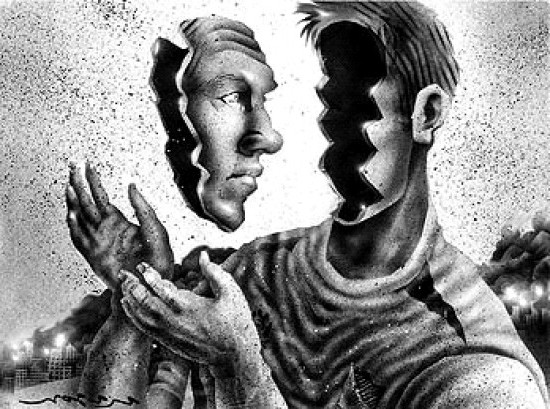
\includegraphics[scale=0.4]{gfx/self-deception.jpg}
	\end{center}
\end{frame}

\begin{frame}
	\begin{center}
		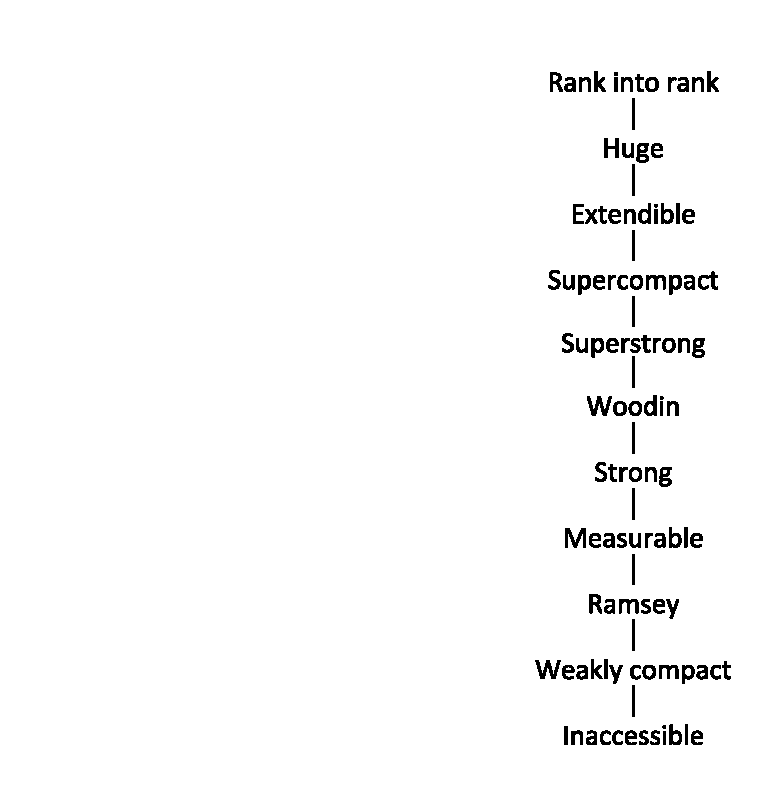
\includegraphics[scale=0.6]{gfx/large_cardinals1.pdf}
	\end{center}
\end{frame}

\begin{frame}
	\begin{center}
		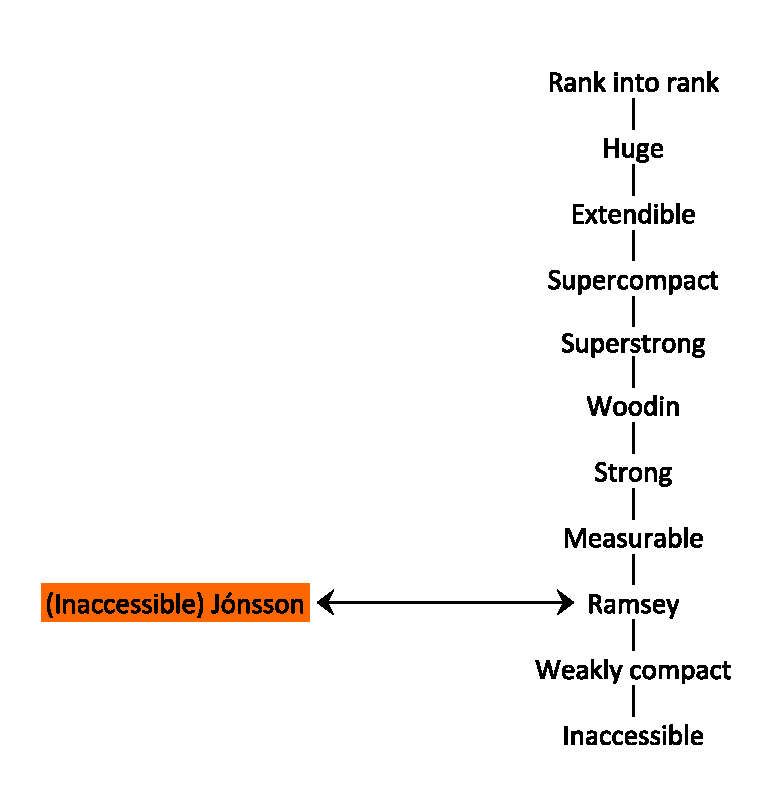
\includegraphics[scale=0.6]{gfx/large_cardinals2.pdf}
	\end{center}
\end{frame}

\begin{frame}
	\begin{center}
		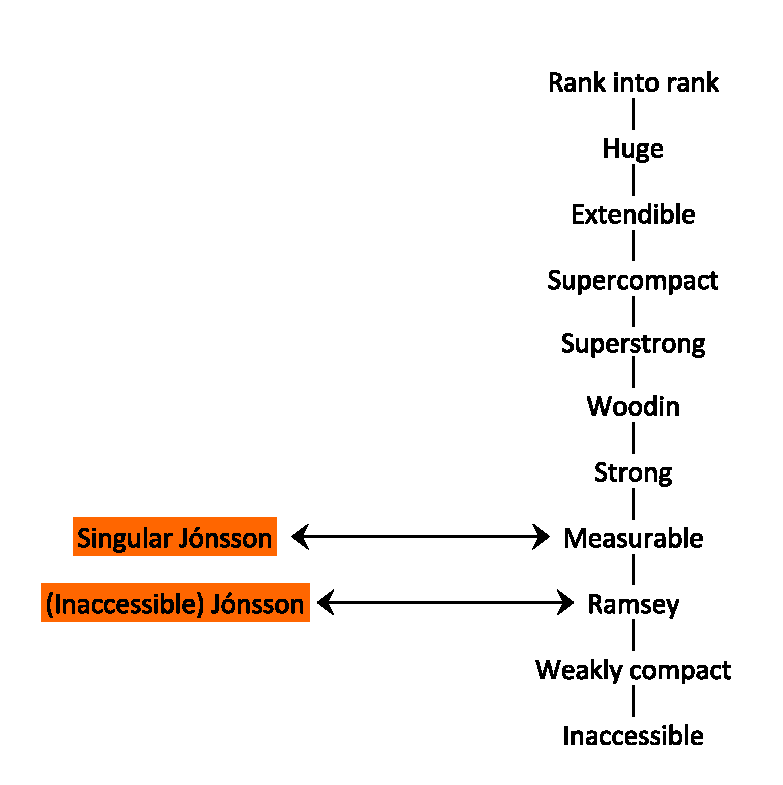
\includegraphics[scale=0.6]{gfx/large_cardinals3.pdf}
	\end{center}
\end{frame}

\begin{frame}
	\begin{center}
		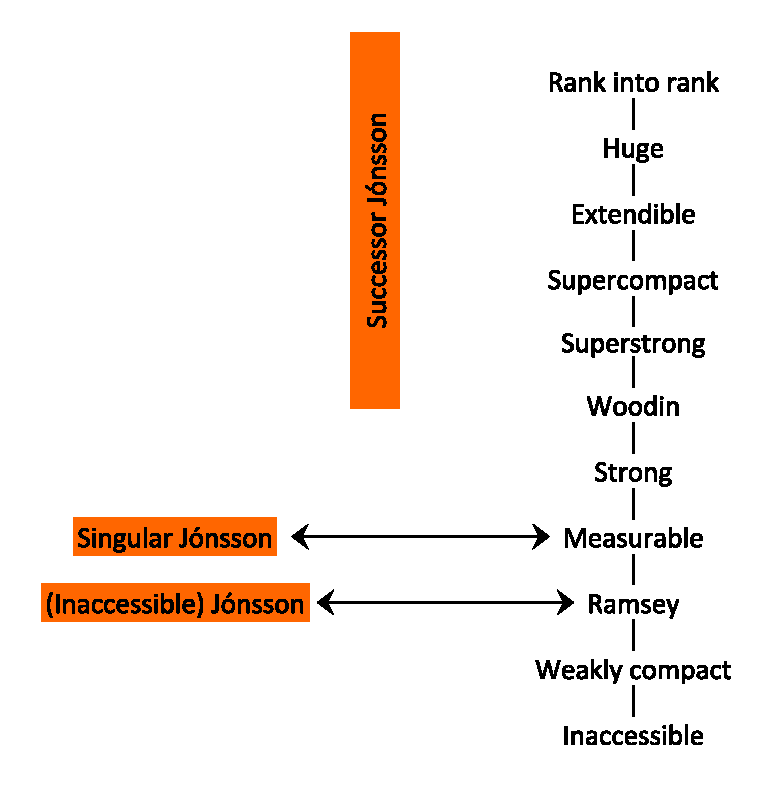
\includegraphics[scale=0.6]{gfx/large_cardinals4.pdf}
	\end{center}
\end{frame}

\begin{frame}
	\begin{center}
		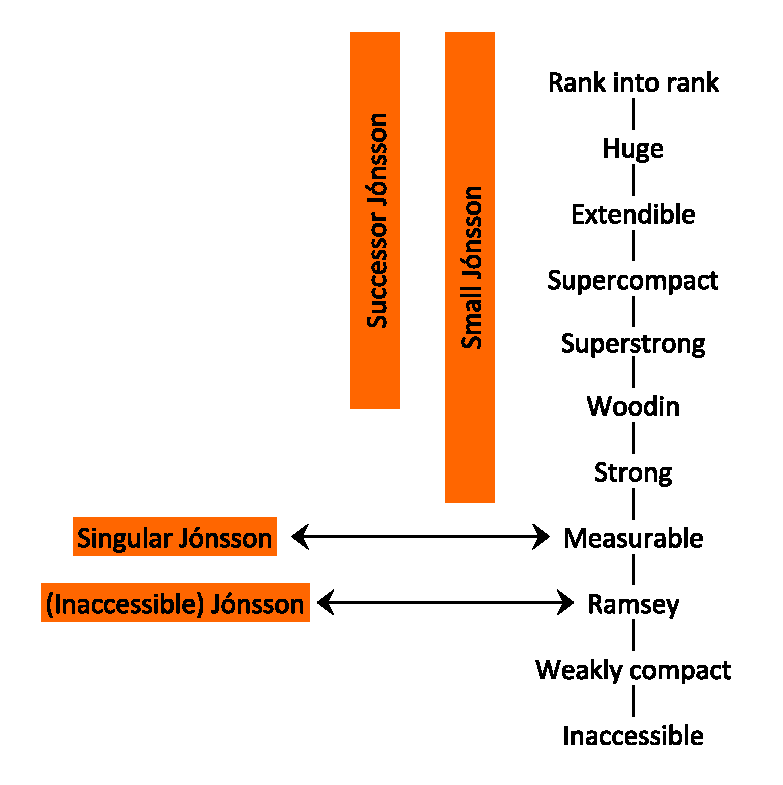
\includegraphics[scale=0.6]{gfx/large_cardinals5.pdf}
	\end{center}
\end{frame}

\begin{frame}
	\begin{center}
		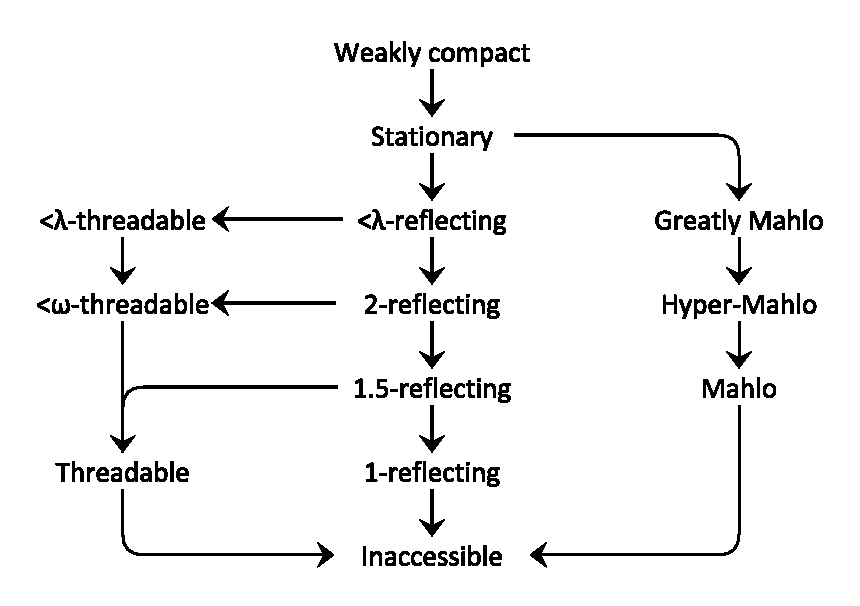
\includegraphics[scale=0.7]{gfx/weakly_compact1.pdf}
	\end{center}
\end{frame}

\begin{frame}
	\begin{center}
		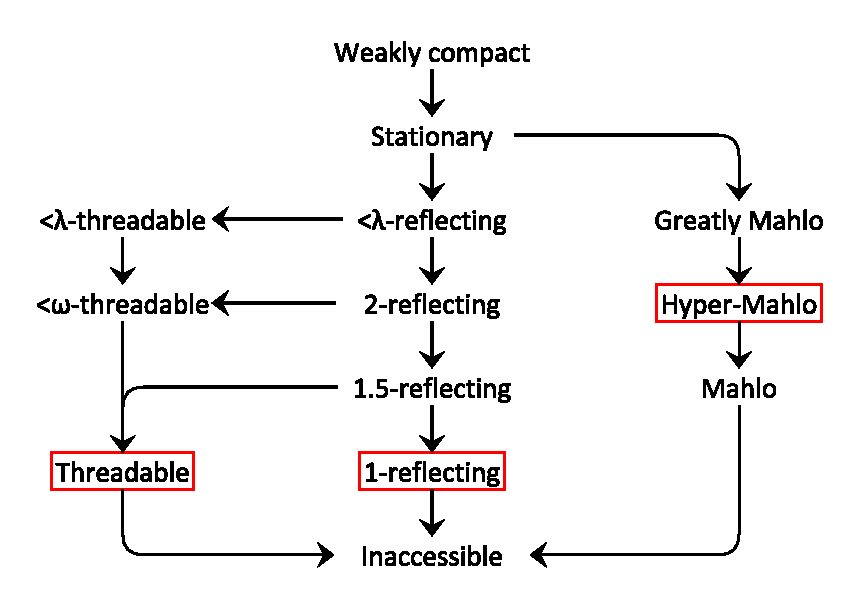
\includegraphics[scale=0.7]{gfx/weakly_compact2.pdf}
	\end{center}
\end{frame}

\begin{frame}
  \begin{center}
		{\Large Thank you for your attention!}\\\vspace{1cm}
		Slides and notes are available at {\color{blue}\href{https://dsnielsen.com/talks/}{dsnielsen.com/talks}}
  \end{center}
\end{frame}

\begin{frame}{References}
	\scriptsize
  \begin{itemize}
		\item Apter ('09): Stationary reflection and level by level equivalence, Colloquium Mathematicum.
		\item Hayut \& Lambie-Hanson ('16): Simultaneous stationary reflection and square sequences, preprint.
		\item Koepke ('88): Some applications of short core models. Annals of Pure and Applied Logic.
		\item Mitchell ('79): Ramsey cardinals and constructibility. The Journal of Symbolic Logic.
		\item Mitchell, Schimmerling \& Steel ('97): The covering lemma up to a Woodin cardinal. Annals of Pure and Applied Logic.
		\item P\v rikr\' y ('70): Changing measurable into accessible cardinals. PhD thesis.
    \item Rinot ('14): Chain conditions of products, and weakly compact cardinals. Bulletin of Symbolic Logic.
    \item Schindler \& Steel ('14): The Core Model Induction (book).
		\item Shelah ('80): On a problem of Kurosh, J\' onsson groups and applications. Studies in Logic and the Foundations of Mathematics.
    \item Shelah ('98): More J�nsson algebras. Archive for Mathematical Logic.
    \item Tryba ('84): On J�nsson cardinals with uncountable cofinality. Israel Journal of Mathematics.
    \item Welch ('98): Some remarks on the maximality of inner models. Logic Colloquium 1998.
  \end{itemize}
\end{frame}

\end{document}
